

\subsection{Subsystem 1 thruster subsystem}

\begin{figure}[h!]
	\centering
 	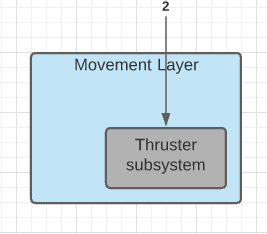
\includegraphics[width=0.60\textwidth]{images/subsystem_movement}
 \caption{Example subsystem description diagram}
\end{figure}

\subsubsection{Assumptions}
We made the assumption that placement of thrusters and general thruster design would be better to copy than to design on our own. We're using our design specifications in accordance with the ArduPilot library documentation.

\subsubsection{Responsibilities}
the responsibility of the thruster subsystem is to move the robot by pushing water through the thrusters. It can also reposition the robot in accordance to the ArduPilot specifications with 8 degrees of freedom.

\subsubsection{Subsystem Interfaces}

\begin {table}[H]
\caption {Subsystem interfaces} 
\begin{center}
    \begin{tabular}{ | p{1cm} | p{6cm} | p{3cm} | p{3cm} |}
    \hline
    ID & Description & Inputs & Outputs \\ \hline
    \#xx & copper wire interface & \pbox{3cm}{electricity} & \pbox{3cm}{kinetic motion}  \\ \hline
    \end{tabular}
\end{center}
\end{table}
